%%%%%%%%%%%%%%%%%%%%%%%%%%%%%%%
%This is the article LaTeX template for RSC journals
%Copyright The Royal Society of Chemistry 2010
%%%%%%%%%%%%%%%%%%%%%%%%%%%%%%%

%\documentclass[8.5pt,twoside,twocolumn]{article}

\documentclass[12pt]{article}
\oddsidemargin -1.2cm
\evensidemargin -1.2cm
\textwidth 18cm
%\oddsidemargin -0.2cm
%\evensidemargin -1.2cm
%\textwidth 16cm
\headheight 1.0in
\topmargin -3.5cm
\textheight 22cm
\usepackage[super,sort&compress,comma]{natbib} 
\usepackage{mhchem}
\usepackage[nomarkers]{endfloat}
\usepackage{siunitx}
\usepackage{times,mathptmx}
% \usepackage{times}
% feel free not to use mathptmx if it causes difficulties
\usepackage{sectsty}
\usepackage{balance} 
\usepackage{comment}
\usepackage{graphicx} %eps figures can be used instead
\usepackage{lastpage}
\usepackage{setspace}
\usepackage[format=plain,justification=raggedright,singlelinecheck=false,font=small,labelfont=bf,labelsep=space]{caption} 
\usepackage{fancyhdr}
\usepackage{multirow}
\usepackage{enumitem}
\usepackage{booktabs}
\usepackage{multicol}
\usepackage{array}
\usepackage{lineno}
\setlength\linenumbersep{0.5cm}
\newcolumntype{H}{>{\setbox0=\hbox\bgroup}c<{\egroup}@{}}
\pagestyle{fancy}


\newcommand{\bra}[2][0]
{\ifthenelse{\equal{#1}{0}}{\left\langle #2 \right|}
{\ifthenelse{\equal{#1}{1}}{\big\langle #2 \big|}
{\ifthenelse{\equal{#1}{2}}{\Big\langle #2 \Big|}
{\ifthenelse{\equal{#1}{3}}{\bigg\langle #2 \bigg|}
{\ifthenelse{\equal{#1}{4}}{\Bigg\langle #2 \Bigg|}
{Error}}}}}
}

% <#2|#3|#4>, #1 gives the size of the bracket
\newcommand{\bracket}[4][0]
{\ifthenelse{\equal{#1}{0}}{\left\langle #2 \middle| #3 \middle| #4 \right\rangle}
{\ifthenelse{\equal{#1}{1}}{\big\langle #2 \big| #3 \big| #4 \big\rangle}
{\ifthenelse{\equal{#1}{2}}{\Big\langle #2 \Big| #3 \Big| #4 \Big\rangle}
{\ifthenelse{\equal{#1}{3}}{\bigg\langle #2 \bigg| #3 \bigg| #4 \bigg\rangle}
{\ifthenelse{\equal{#1}{4}}{\Bigg\langle #2 \Bigg| #3 \Bigg| #4 \Bigg\rangle}
{Error}}}}}
}

% <#2|#3>, #1 gives the size of the bracket
\newcommand{\braket}[3][0]
{\ifthenelse{\equal{#1}{0}}{\left\langle #2 \middle| #3 \right\rangle}
{\ifthenelse{\equal{#1}{1}}{\big\langle #2 \big| #3 \big\rangle}
{\ifthenelse{\equal{#1}{2}}{\Big\langle #2 \Big| #3 \Big\rangle}
{\ifthenelse{\equal{#1}{3}}{\bigg\langle #2 \bigg| #3 \bigg\rangle}
{\ifthenelse{\equal{#1}{4}}{\Bigg\langle #2 \Bigg| #3 \Bigg\rangle}
{Error}}}}}
}

% |#2>, #1 gives the size of the bracket
\newcommand{\ket}[2][0]
{\ifthenelse{\equal{#1}{0}}{\left| #2 \right\rangle}
{\ifthenelse{\equal{#1}{1}}{\big| #2 \big\rangle}
{\ifthenelse{\equal{#1}{2}}{\Big| #2 \Big\rangle}
{\ifthenelse{\equal{#1}{3}}{\bigg| #2 \bigg\rangle}
{\ifthenelse{\equal{#1}{4}}{\Bigg| #2 \Bigg\rangle}
{Error}}}}}
}


\begin{document}
\thispagestyle{plain}
\fancypagestyle{plain}{
\fancyhead[L]{
\includegraphics[height=8pt]{headers/LH}}
\fancyhead[C]{\hspace{-1cm}
\includegraphics[height=20pt]{headers/CH}}
\fancyhead[R]{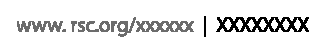
\includegraphics[height=10pt]{headers/RH}\vspace{-0.2cm}}
\renewcommand{\headrulewidth}{1pt}}
\renewcommand{\thefootnote}{\fnsymbol{footnote}}
\renewcommand\footnoterule{\vspace*{1pt}% 
\hrule width 3.4in height 0.4pt \vspace*{5pt}} 
\setcounter{secnumdepth}{5}



\makeatletter 
\def\subsubsection{\@startsection{subsubsection}{3}{10pt}{-1.25ex plus -1ex minus -.1ex}{0ex plus 0ex}{\normalsize\bf}} 
\def\paragraph{\@startsection{paragraph}{4}{10pt}{-1.25ex plus -1ex minus -.1ex}{0ex plus 0ex}{\normalsize\textit}} 
\renewcommand\@biblabel[1]{#1}            
\renewcommand\@makefntext[1]% 
{\noindent\makebox[0pt][r]{\@thefnmark\,}#1}
\makeatother 
\renewcommand{\figurename}{\small{Fig.}~}
\sectionfont{\large}
\subsectionfont{\normalsize} 

\fancyfoot{}
\fancyfoot[LO,RE]{\vspace{-7pt}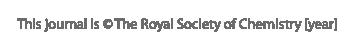
\includegraphics[height=9pt]{headers/LF}}
\fancyfoot[CO]{\vspace{-7.2pt}\hspace{12.2cm}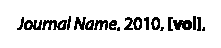
\includegraphics{headers/RF}}
\fancyfoot[CE]{\vspace{-7.5pt}\hspace{-13.5cm}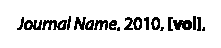
\includegraphics{headers/RF}}
\fancyfoot[RO]{\footnotesize{\sffamily{1--\pageref{LastPage} ~\textbar  \hspace{2pt}\thepage}}}
\fancyfoot[LE]{\footnotesize{\sffamily{\thepage~\textbar\hspace{3.45cm} 1--\pageref{LastPage}}}}
\fancyhead{}
\renewcommand{\headrulewidth}{1pt} 
\renewcommand{\footrulewidth}{1pt}
\setlength{\arrayrulewidth}{1pt}
\setlength{\columnsep}{6.5mm}
\setlength\bibsep{1pt}

%\linenumbers
\noindent\LARGE{\textbf{
%Using Conventional Density Functionals to Simulate X-Ray Absorption Spectra: With Applications to Adenine and Thymine Photoabsorption Spectra
Simulation of X-Ray Absorption Spectra with Orthogonality Constrained Density Functional Theory
}}
\vspace{0.6cm}

\noindent\large{\textbf{Wallace D. Derricotte and Francesco A. Evangelista$^{\ast}$}}\vspace{0.5cm}
%Please note that \ast indicates the corresponding author(s) but no footnote text is required. 


\noindent\textit{\small{\textbf{Received Xth XXXXXXXXXX 20XX, Accepted Xth XXXXXXXXX 20XX\newline
First published on the web Xth XXXXXXXXXX 200X}}}

\noindent \textbf{\small{DOI: 10.1039/b000000x}}
\vspace{0.6cm}
\section*{Supplementary Materials}
\begin{table}
\centering
\caption{Optimized cartesian geometry of adenine used for simulation of NEXAS spectra optimized at the B3LYP/def2-TZVP level of theory using the \textsc{psi4} {\textit{ab initio}} quantum chemistry package.}
\begin{tabular}{cccc}
\hline
\hline
    C     &      -1.970585664532  &   -1.395137524338  &   -0.045467117394 \vspace{0.3cm}\\
    N      &      -1.881922764968  &   -0.101178970901 &    -0.187746915294 \vspace{0.3cm}\\
    C       &     -0.530036651175  &    0.162042066892  &   -0.075212958513 \vspace{0.3cm}\\
    C       &      0.194518534413  &   -1.008769908818  &    0.138884730519 \vspace{0.3cm}\\
    N        &    -0.752839154291  &   -2.003591795126 &     0.155019478510 \vspace{0.3cm}\\
    H       &     -0.575304730981&     -2.985001122876  &    0.288894532977 \vspace{0.3cm}\\
    H      &      -2.887084126393 &    -1.963704194624  &   -0.076026591074 \vspace{0.3cm}\\
    C         &    0.220821847281  &    1.350420528553  &   -0.134877528376 \vspace{0.3cm}\\
    N        &     1.548880751460  &    1.275830644080 &     0.014725285193 \vspace{0.3cm}\\
    C        &     2.109044063853   &   0.076787593229   &   0.214691629565 \vspace{0.3cm}\\
    N        &     1.515353675426  &   -1.110912425553  &    0.290953400869 \vspace{0.3cm}\\
    H      &       3.187892320597 &     0.080293623862  &    0.328711091758 \vspace{0.3cm}\\
    N       &     -0.350021924019   &   2.556054469300  &   -0.336758184831 \vspace{0.3cm}\\
    H       &     -1.344255431781  &    2.632817141374  &   -0.451219656473 \vspace{0.3cm}\\
    H      &       0.231906121724   &   3.373853460732  &   -0.370895998201 \\
    \hline
    \hline
    \end{tabular}
\end{table}
\begin{table}
\centering
\caption{ Optimized cartesian geometry of thymine used for simulation of NEXAS spectra optimized at the B3LYP/def2-TZVP level of theory using the \textsc{psi4} {\textit{ab initio}} quantum chemistry package.}
\begin{tabular}{cccc}
\hline
\hline
    C      &     -1.246495845834  &   0.412642804754 &   -0.003573103168 \vspace{0.3cm}\\
    C      &     -2.507237287316   &  1.217084061874  &  -0.011848989295 \vspace{0.3cm}\\
    H      &     -3.117873132937   &  1.004161896948  &  -0.892346853646 \vspace{0.3cm}\\
    H       &    -2.252332058556   &  2.276314275673  &  -0.024950360779 \vspace{0.3cm}\\
    H     &      -3.115843391524   &  1.025528612536   &  0.874939447790 \vspace{0.3cm}\\
    C     &      -1.217630214628  &  -0.931441458484  &   0.012635606229 \vspace{0.3cm}\\
    N      &     -0.056489889005  &  -1.654192870252  &   0.020052122522 \vspace{0.3cm}\\
    C      &      1.197028093408  &  -1.083944060777   &  0.011743762351 \vspace{0.3cm}\\
    N      &      1.154191491462  &   0.288466721271  &  -0.004799899183 \vspace{0.3cm}\\
    C      &      0.033038734047  &   1.117787686433  &  -0.013561659185 \vspace{0.3cm}\\
    H       &     2.050520064174  &   0.753906293046  &  -0.011435103920 \vspace{0.3cm}\\
    O       &     0.171793664591  &   2.321663419892  &  -0.028248779210 \vspace{0.3cm}\\
    O       &     2.217898772608   & -1.730464525441  &   0.018397425821 \vspace{0.3cm}\\
    H       &    -2.125375374356  &  -1.524102636497  &   0.020825176486 \vspace{0.3cm}\\
    H       &    -0.070123074504 &   -2.660021414373  &   0.032219688224 \\
    \hline
    \hline
    \end{tabular}
\end{table}
   \begin{table}
   \footnotesize
 \centering
          \caption{Calculated and experimental thymine oxygen core excitation energies in eV are shown in the table. All computations are performed using the def2-TZVP basis set and B3LYP functional. The largest contribution to the particle orbital ($\phi_p$) with reference to the ground state valence set is reported along with the hole orbital ($\phi_h$) for each transition. Relative oscillator strengths (f$_{rel}$) are also reported}
     \begin{tabular}{c@{\hskip 0.22in}c@{\hskip 0.22in}c@{\hskip 0.22in}c@{\hskip 0.52in}c@{\hskip 0.22in}c@{\hskip 0.22in}c}
     \hline
     \hline
   \multicolumn{4}{c}{OCDFT} &\multicolumn{2}{c}{Experiment} \\
   \hline
 $\phi_h$ &  $\phi_p$ & $\omega_{fi}$ & f$_{rel}$ & Peak &  $\omega_{fi}$   \\
   \hline
    O$_2$
 &   81.8$\%$ $\pi_1^*$  & 531.05 & 1.000 & A  & 531.4
 \vspace{0.1in}\\
    O$_1$
 &   64.0$\%$ $\pi_2^*$  & 532.08 & 0.968 & B & 532.3
 \vspace{0.1in}\\
    O$_1$
 &   71.2$\%$ $\pi_1^*$  & 533.38 & 0.146 & \multirow{2}{*}{B$^{\prime}$} & \multirow{2}{*}{$\approx$ 533.8}  \\
    O$_2$
 &   78.3$\%$ $\pi_2^*$  & 533.75 & 0.162 
 \vspace{0.1in}\\
    O$_1$
 &   77.0$\%$ $\rm D_1$  & 534.74 & 0.008  & \multirow{9}{*}{C} & \multirow{9}{*}{535.7} \\
    O$_2$
 &   65.9$\%$ $\rm D_1$  & 534.85 & 0.042 \\
    O$_2$
 &   44.1$\%$ $\rm D_3$  & 535.28 & 0.020 \\
    O$_1$
 &   69.5$\%$ $\rm D_3$  & 535.46 & 0.098 \\
    O$_2$
 &   60.8$\%$ $\rm D_2$  & 535.53 & 0.085 \\
    O$_1$
 &   76.0$\%$ $\pi_3^*$  & 536.12 & 0.222 \\
    O$_2$
 &   69.0$\%$ $\pi_3^*$  & 536.24 & 0.104 \\
    O$_2$
 &   86.3$\%$ $\rm D_4$  & 536.34 & 0.052 \\
    O$_1$
 &   76.3$\%$ $\rm D_2$  & 536.60 & 0.039 
 \vspace{0.1in}\\
    O$_2$
 &   44.4$\%$ $\rm D_6$  & 537.02 & 0.024 & \multirow{6}{*}{D} & \multirow{6}{*}{537.1} \\
    O$_1$
 &   83.5$\%$ $\rm D_4$  & 537.10 & 0.047 \\
    O$_2$
 &   63.7$\%$ $\rm D_5$  & 537.21 & 0.021 \\
    O$_1$
 &   35.6$\%$ $\rm D_7$   & 537.45 & 0.054 \\
    O$_2$
 &   44.0$\%$ $\rm D_7$   & 537.67 & 0.073 \\
    O$_1$
 &   43.6$\%$ $\rm D_5$  & 537.72 & 0.036 
 \vspace{0.1in}\\
    O$_1$
 &   70.7$\%$ $\rm D_6$  & 538.49 & 0.058 \\
   \end{tabular}
   \label{table: thymine_k_oxygen}
\end{table}
        \begin{table}
        \footnotesize
 \centering
   \caption{Calculated and experimental thymine nitrogen core excitation energies in eV are shown in the table. All computations are performed using the def2-TZVP basis set and B3LYP functional. The largest contribution to the particle orbital ($\phi_p$) with reference to the ground state valence set is reported along with the hole orbital ($\phi_h$) for each transition. Relative oscillator strengths (f$_{rel}$) are also reported}
     \begin{tabular}{c@{\hskip 0.22in}c@{\hskip 0.22in}c@{\hskip 0.22in}c@{\hskip 0.52in}c@{\hskip 0.22in}c@{\hskip 0.22in}c}
     \hline
     \hline
   \multicolumn{4}{c}{OCDFT} &\multicolumn{2}{c}{Experiment} \\
   \hline
 $\phi_h$ &  $\phi_p$ & $\omega_{fi}$ & f$_{rel}$ & Peak &  $\omega_{fi}$   \\
   \hline
    N$_4$
 &   81.8$\%$ $\pi_1^*$  & 401.18 & 1.000 & \multirow{2}{*}{A} & \multirow{2}{*}{401.7} \\
    N$_3$
 &   64.0$\%$ $\pi_2^*$  & 401.76 & 0.805 
 \vspace{0.1in}\\
    N$_4$
 &   78.3$\%$ $\pi_2^*$  & 402.50 & 0.087 & \multirow{3}{*}{B} & \multirow{3}{*}{402.7}\\
    N$_3$
 &   77.0$\%$ $\rm D_1$  & 403.09 & 0.863 \\
    N$_4$
 &   65.9$\%$ $\rm D_1$  & 403.33 & 0.765 
 \vspace{0.1in}\\
    N$_4$
 &   44.1$\%$ $\rm D_3$  & 404.17 & 0.912 & C & 404.1 
 \vspace{0.1in}\\
    N$_4$
 &   60.8$\%$ $\rm D_2$  & 404.94 & 0.144 & \multirow{7}{*}{D} & \multirow{6}{*}{405.5}\\
    N$_3$
 &   69.5$\%$ $\rm D_3$  & 405.09 & 0.374 \\
    N$_4$
 &   86.3$\%$ $\rm D_4$  & 405.31 & 0.864 \\
    N$_3$
 &   76.0$\%$ $\pi_3^*$  & 405.41 & 0.333 \\
    N$_4$
 &   69.0$\%$ $\pi_3^*$  & 405.62 & 0.183 \\
    N$_3$
 &   71.2$\%$ $\pi_1^*$  & 405.67 & 0.490 \\
    N$_3$
 &   76.3$\%$ $\rm D_2$  & 405.76 & 0.177 \\
 \end{tabular}
   \label{table: thymine_k_nitrogen}
\end{table}
      \begin{table}
      \footnotesize
 \centering
    \caption{Calculated and experimental thymine carbon core excitation energies in eV are shown in the table. All computations are performed using the def2-TZVP basis set and B3LYP functional. The largest contribution to the particle orbital ($\phi_p$) with reference to the ground state valence set is reported along with the hole orbital ($\phi_h$) for each transition. Relative oscillator strengths (f$_{rel}$) are also reported}
     \begin{tabular}{c@{\hskip 0.22in}c@{\hskip 0.22in}c@{\hskip 0.22in}c@{\hskip 0.52in}c@{\hskip 0.22in}c@{\hskip 0.22in}c}
     \hline
     \hline
   \multicolumn{4}{c}{OCDFT} &\multicolumn{2}{c}{Experiment} \\
   \hline
 $\phi_h$ &  $\phi_p$ & $\omega_{fi}$ & f$_{rel}$ & Peak &  $\omega_{fi}$   \\
   \hline
    C$_8$
 &   92.1$\%$ $\pi_1^*$  & 284.90 & 0.372 & A & 284.9  
 \vspace{0.1in} \\
    C$_7$
 &   95.9$\%$ $\pi_1^*$  & 285.98 & 0.698 & B & 285.9
 \vspace{0.1in} \\
    C$_9$
 &   75.4$\%$ $\pi_2^*$  & 286.56 & 0.036 & \multirow{5}{*}{C} & \multirow{5}{*}{287.8} \\
    C$_8$
 &   97.6$\%$ $\pi_2^*$  & 287.33 & 0.171 \\
    C$_6$
 &   81.8$\%$ $\pi_1^*$  & 287.68 & 0.792 \\
    C$_9$
 &   89.9$\%$ $\pi_1^*$  & 287.92 & 0.117 \\
    C$_8$
 &   48.1$\%$ $\rm D_3$  & 288.19 & 0.006 
 \vspace{0.1in} \\
    C$_9$
 &   87.7$\%$ $\rm D_1$  & 288.46 & 0.229 & \multirow{9}{*}{D} & \multirow{9}{*}{289.4} \\
    C$_8$
 &   53.9$\%$ $\rm D_1$  & 288.94 & 0.037 \\
    C$_9$
 &   85.1$\%$ $\rm D_3$  & 289.01 & 0.158 \\
    C$_7$
 &   94.2$\%$ $\pi_2^*$  & 289.06 & 0.289 \\
    C$_5$
 &   64.0$\%$ $\pi_2^*$  & 289.14 & 1.000 \\
    C$_8$
 &   32.5$\%$ $\rm D_3$  & 289.17 & 0.017 \\
    C$_7$
 &   90.3$\%$ $\rm D_1$  & 289.22 & 0.001 \\
    C$_9$
 &   63.1$\%$ $\pi_3^*$  & 289.26 & 0.333 \\
    C$_9$
 &   49.5$\%$ $\rm D_2$  & 289.31 & 0.375 
 \vspace{0.1in}\\
    C$_8$
 &   67.1$\%$ $\rm D_2$  & 289.67 & 0.082 \\
    C$_8$
 &   77.0$\%$ $\rm D_4$  & 289.68 & 0.105 \\
    C$_6$
 &   78.3$\%$ $\pi_2^*$  & 289.94 & 0.135 
 \vspace{0.1in}\\
    C$_9$
 &   75.4$\%$ $\rm D_4$  & 290.14 & 0.023 & \multirow{6}{*}{E} &  \multirow{6}{*}{290.7} \\
    C$_8$
 &   33.3$\%$ $\rm D_5$  & 290.31 & 0.119 \\
    C$_5$
 &   71.2$\%$ $\pi_1^*$  & 290.33 & 0.029 \\
    C$_9$
 &   30.5$\%$ $\rm D_5$  & 290.43 & 0.047 \\
    C$_7$
 &   71.6$\%$ $\rm D_3$  & 290.44 & 0.050 \\
    C$_7$
 &   41.5$\%$ $\rm D_2$  & 290.54 & 0.041 
 \vspace{0.1in}\\
    C$_8$
 &   38.1$\%$ $\rm D_6$  & 290.80 & 0.093 \\
    C$_9$
 &   24.4$\%$ $\rm D_6$  & 291.12 & 0.076 \\
    C$_8$
 &   61.2$\%$ $\rm D_7$  & 291.13 & 0.024 \\
    C$_7$
 &   45.5$\%$ $\pi_3^*$  & 291.42 & 0.018 \\
    C$_7$
 &   83.1$\%$ $\rm D_4$  & 291.44 & 0.001 \\
    C$_9$
 &   24.8$\%$ $\rm D_5$  & 291.45 & 0.289 \\
    C$_6$
 &   65.9$\%$ $\rm D_1$  & 291.59 & 0.036 \\
    C$_7$
 &   44.3$\%$ $\rm D_5$  & 291.83 & 0.055 \\
 \end{tabular}
   \label{table: thymine_k_carbon}
\end{table}
  \begin{table}
  \footnotesize
 \centering
    \caption{Calculated and experimental adenine nitrogen core excitation energies in eV are shown in the table. All computations are performed using the def2-TZVP basis set and B3LYP functional. The largest contribution to the particle orbital ($\phi_p$) with reference to the ground state valence set is reported along with the hole orbital ($\phi_h$) for each transition. Relative oscillator strengths (f$_{rel}$) are also reported}
     \begin{tabular}{c@{\hskip 0.22in}c@{\hskip 0.22in}c@{\hskip 0.22in}c@{\hskip 0.52in}c@{\hskip 0.22in}c@{\hskip 0.22in}c}
     \hline
     \hline
   \multicolumn{4}{c}{OCDFT} &\multicolumn{2}{c}{Experiment} \\
   \hline
 $\phi_h$ &  $\phi_p$ & $\omega_{fi}$ & f$_{rel}$ & Peak &  $\omega_{fi}$   \\
   \hline
    N$_4$
 &   81.0$\%$ $\pi_1^*$  & 399.14 & 0.851 & \multirow{3}{*}{A} & \multirow{3}{*}{399.5} \\
    N$_3$
 &   63.7$\%$ $\pi_1^*$  & 399.28 & 0.926 \\
    N$_5$
 &   92.6$\%$ $\pi_2^*$  & 399.42 & 1.000 
\vspace{0.1in}\\
    N$_5$
 &   92.4$\%$ $\pi_1^*$  & 399.69 & 0.002 & \multirow{2}{*}{A$^{\prime}$} & \multirow{2}{*}{$\approx$ 400.4}  \\
    N$_4$
 &   98.9$\%$ $\pi_2^*$
 & 400.39 & 0.022 
 \vspace{0.1in}\\
    N$_3$
 &   81.6$\%$ $\pi_2^*$  & 401.21 & 0.109 & B$^{\prime}$ & 401.3 
 \vspace{0.1in}\\
    N$_2$
 &   82.1$\%$ $\pi_1^*$  & 401.43 & 0.364 & \multirow{9}{*}{B} & \multirow{9}{*}{401.9}\\
    N$_3$
 &   66.2$\%$ $\pi_3^*$  & 401.79 & 0.145 \\
    N$_1$
 &   69.3$\%$ $\pi_1^*$  & 401.81 & 0.594 \\
    N$_4$
 &   77.4$\%$ $\pi_3^*$  & 401.95 & 0.184 \\
    N$_5$
 &   56.7$\%$ $\pi_3^*$  & 402.10 & 0.017 \\
    N$_5$
 &   34.7$\%$ $\pi_3^*$  & 402.15 & 0.013 \\
    N$_2$
 &   78.4$\%$ $\rm D_3$  & 402.27 & 0.204 \\
    N$_4$
 &   80.2$\%$ $\rm D_2$  & 402.36 & 0.003 \\
    N$_3$
 &   90.2$\%$ $\rm D_2$  & 402.42 & 0.012 
 \vspace{0.1in}\\
    N$_4$
 &   83.4$\%$ $\rm D_3$  & 402.73 & 0.038 & \multirow{10}{*}{C} & \multirow{10}{*}{403.0}\\
    N$_3$
 &   69.0$\%$ $\rm D_3$  & 402.80 & 0.008 \\
    N$_5$
 &   36.4$\%$ $\rm D_3$  & 402.80 & 0.049 \\
    N$_1$
 &   74.8$\%$ $\pi_2^*$  & 403.08 & 0.122 \\
    N$_5$
 &   39.1$\%$ $\rm D_5$  & 403.18 & 0.030 \\
    N$_4$
 &   48.5$\%$ $\rm D_4$  & 403.22 & 0.033 \\
    N$_1$
 &   87.2$\%$ $\rm D_2$  & 403.25 & 0.418 \\
    N$_3$
 &   80.4$\%$ $\rm D_4$  & 403.32 & 0.074 \\
    N$_2$
 &   57.1$\%$ $\rm D_6$  & 403.34 & 0.918 \\
    N$_5$
 &   91.1$\%$ $\rm D_6$  & 403.38 & 0.052 
 \vspace{0.1in}\\
    N$_4$
 &   61.7$\%$ $\rm D_6$  & 403.67 & 0.007 \\
    N$_3$
 &   77.6$\%$ $\rm D_5$  & 403.72 & 0.007 \\
    N$_5$
 &   61.6$\%$  $\rm D_7$ & 403.79 & 0.073 \\
    N$_1$
 &   77.2$\%$ $\pi_3^*$  & 403.97 & 0.083 \\
    N$_4$
 &   37.1$\%$ $\rm D_7$  & 404.07 & 0.040 \\
    N$_5$
 &   36.3$\%$ $\rm D_4$  & 404.20 & 0.008 \\
    N$_4$
 &   39.8$\%$ $\rm D_7$ & 404.24 & 0.022 \\
    N$_2$
 &   94.8$\%$ $\pi_3^*$  & 404.33 & 0.038 \\
    N$_3$
 &   42.3$\%$ $\rm D_8$  & 404.44 & 0.023 \\
    N$_2$
 &   87.1$\%$ $\pi_2^*$  & 404.55 & 0.011 \\
    N$_3$
 &   59.8$\%$ $\rm D_6$  & 404.71 & 0.059 \\
    N$_5$
 &   29.0$\%$ $\rm D_5$  & 404.73 & 0.031 \\
    N$_4$
 &   91.9$\%$ $\rm D_{10}$  & 404.79 & 0.253 \\
    N$_2$
 &   56.6$\%$ $\rm D_2$  & 404.97 & 0.115 \\
 \hline
 \hline
   \end{tabular}
 \label{fig: adenine_k_nitrogen}
\end{table}
  \begin{table}
  \footnotesize
 	\centering
\caption{Calculated and experimental adenine carbon core excitation energies in eV are shown in the table. All computations are performed using the def2-TZVP basis set and B3LYP functional. The largest contribution to the particle orbital ($\phi_p$) with reference to the ground state valence set is reported along with the hole orbital ($\phi_h$) for each transition. Relative oscillator strengths (f$_{rel}$) are also reported}
     \begin{tabular}{c@{\hskip 0.22in}c@{\hskip 0.22in}c@{\hskip 0.22in}c@{\hskip 0.52in}c@{\hskip 0.22in}c@{\hskip 0.22in}c}
     \hline
     \hline
   \multicolumn{4}{c}{OCDFT} &\multicolumn{2}{c}{Experiment} \\
   \hline
 $\phi_h$ &  $\phi_p$ & $\omega_{fi}$ & f$_{rel}$ & Peak &  $\omega_{fi}$   \\
   \hline
    C$_{10}$
 &   92.6$\%$ $\pi_2^*$  & 286.32 & 0.298 & \multirow{2}{*}{A} & \multirow{2}{*}{286.4}\\
    C$_9$
 &   81.0$\%$ $\pi_1^*$  & 286.46 & 0.936 
 \vspace{0.1in}\\
    C$_{10}$
 &   92.4$\%$ $\pi_1^*$  & 286.71 & 0.260 &  \multirow{2}{*}{B} &  \multirow{2}{*}{286.8} \\
    C$_7$
 &   82.1$\%$ $\pi_1^*$  & 286.86 & 0.893 
 \vspace{0.1in}\\
    C$_6$
 &   69.3$\%$ $\pi_1^*$  & 287.27 & 1.000 &  \multirow{2}{*}{C} &  \multirow{2}{*}{287.4}\\
    C$_8$
 &   63.7$\%$ $\pi_1^*$  & 287.41 & 0.961 
 \vspace{0.1in}\\
    C$_8$
 &   81.6$\%$ $\pi_2^*$  & 287.86 & 0.000 &  \multirow{3}{*}{C$^{\prime}$} &  \multirow{3}{*}{$\approx$ 288.0}\\
    C$_{10}$
 &   34.7$\%$ $\pi_3^*$  & 287.93 & 0.092 \\
    C$_9$
 &   98.9$\%$ $\pi_2^*$
 & 288.02 & 0.026 
 \vspace{0.1in}\\
    C$_6$
 &   74.8$\%$ $\pi_2^*$  & 288.78 & 0.008 & \multirow{5}{*}{D} & \multirow{5}{*}{289.0} \\
    C$_{10}$
 &   56.7$\%$ $\pi_3^*$  & 288.89 & 0.006 \\
    C$_7$
 &   78.4$\%$ $\rm D_3$  & 288.91 & 0.001 \\
    C$_{10}$
 &   36.4$\%$ $\rm D_3$  & 289.16 & 0.038 \\
    C$_8$
 &   66.2$\%$ $\pi_3^*$  & 289.21 & 0.014 
 \vspace{0.1in}\\
    C$_9$
 &   77.4$\%$ $\pi_3^*$  & 289.41 & 0.016 & \multirow{3}{*}{E} \\
    C$_7$
 &   87.1$\%$ $\pi_2^*$  & 289.43 & 0.042 \\
    C$_7$
 &   57.1$\%$ $\rm D_6$  & 289.66 & 0.329 
 \vspace{0.1in}\\
    C$_{10}$
 &   39.1$\%$ $\rm D_5$  & 289.82 & 0.029 & \multirow{5}{*}{F} \\
    C$_9$
 &   80.2$\%$ $\rm D_2$  & 289.98 & 0.266 \\
    C$_8$
 &   90.2$\%$ $\rm D_2$  & 290.06 & 0.044 \\
    C$_9$
 &   83.4$\%$ $\rm D_3$  & 290.14 & 0.166 \\
    C$_6$
 &   87.2$\%$ $\rm D_2$  & 290.15 & 0.035 
 \vspace{0.1in}\\
    C$_7$
 &   94.8$\%$ $\pi_3^*$  & 290.36 & 0.086  & \multirow{8}{*}{G} \\
    C$_{10}$
 &   91.1$\%$ $\rm D_6$  & 290.37 & 0.020 \\
    C$_{10}$
 &   61.6$\%$ $\rm D_7$  & 290.42 & 0.031 \\
    C$_9$
 &   48.5$\%$ $\rm D_4$  & 290.45 & 0.014 \\
    C$_8$
 &   69.0$\%$ $\rm D_3$  & 290.61 & 0.010 \\
    C$_6$
 &   77.2$\%$ $\pi_3^*$  & 290.66 & 0.060 \\
    C$_7$
 &   56.6$\%$ $\rm D_2$  & 290.77 & 0.064 \\
    C$_9$
 &   61.7$\%$ $\rm D_6$  & 290.94 & 0.018 \\
 \hline
 \hline
   \end{tabular}
   \label{table: adenine_k_carbon}
\end{table}
\end{document}